%==============================================================================
% Voorbeeld gebruik documentklasse hogent-article
%==============================================================================
%
% Compileren in TeXstudio:
%
% - Zorg dat Biber de bibliografie compileert (en niet Biblatex)
%   Options > Configure > Build > Default Bibliography Tool: "txs:///biber"
% - F5 om te compileren en het resultaat te bekijken.
% - Als de bibliografie niet zichtbaar is, probeer dan F5 - F8 - F5
%   Met F8 compileer je de bibliografie apart.
%
% Als je JabRef gebruikt voor het bijhouden van de bibliografie, zorg dan
% dat je in ``biblatex''-modus opslaat: File > Switch to BibLaTeX mode.

\documentclass{hogent-article}
\usepackage[dutch]{babel} % Voor vultekst
 \usepackage{graphicx}
%------------------------------------------------------------------------------
% Metadata over het artikel
%------------------------------------------------------------------------------

%---------- Titel & auteur ----------------------------------------------------

% TODO: geef werktitel van je eigen voorstel op
\PaperTitle{De invloed van fysieke gezondheid op wiskundige geletterdheid bij tweedejaarsstudenten Toegepaste Informatica}
% TODO: geef op welk soort artikel dit is
% Dit is typisch de opdracht en het vak waarvoor dit artikel geschreven is, bv.
% ``Verslag onderzoeksproject Onderzoekstechnieken 2018-2019''
\PaperType{Eindrapport Onderzoekstechnieken 2020-2021}

% TODO: vul je eigen naam in als auteur, geef ook je emailadres mee!
\Authors{Collin Verhaeghe\textsuperscript{1}, Benjamin Schoeters\textsuperscript{2}, Ilya Mikhaylov\textsuperscript{3}, Kasper Van Remoortere\textsuperscript{4}, Wesley Maebe\textsuperscript{5}} % Authors

% TODO: vul de naam van je co-promotor in.
% Als het hier gaat om een voorstel voor de bachelorproef, dan ben je hier
% verplicht de naam van je co-promotor in te vullen. Zoniet, dan kan je het
% leeg laten.
\CoPromotor{}

% Contactinfo: Geef hier de contactgegevens van elke auteur van het artikel (en
% indien van toepassing ook van de co-promotor).
\affiliation{
  \textsuperscript{1} \href{mailto:collin.verhaeghe@student.hogent.be}{collin.verhaeghe@student.hogent.be}}
\affiliation{
  \textsuperscript{2} \href{mailto:benjamin.schoeters@student.hogent.be}{benjamin.schoeters@student.hogent.be}}
\affiliation{
\textsuperscript{3} \href{mailto:ilya.mikhaylov@student.hogent.be}{ilya.mikhaylov@student.hogent.be}}
\affiliation{
\textsuperscript{4} \href{mailto:kasper.vanremoortere@student.hogent.be}{kasper.vanremoortere@student.hogent.be}}\affiliation{
\textsuperscript{5} \href{mailto:wesley.maebe@student.hogent.be}{wesley.maebe@student.hogent.be}}

%---------- Abstract ----------------------------------------------------------

\Abstract{De literatuur suggereert dat fysieke activiteit en middelengebruik de academische prestaties van studenten beïnvloedt, maar is niet doorslaggevend over de richting ervan. Deze studie beoogt deze stelling te onderzoeken voor prestaties met betrekking tot wiskundige geletterdheid. In 2020 werden tweedejaars studenten toegepaste informatica (n=217) ondervraagd naar hun wiskundige resultaten en een reeks eigenschappen waarmee hun fysieke gezondheid wordt bepaald. Meer bepaald werd een meting genomen van alcohol, sigarettengebruik, fysieke activiteit en de Body Mass Index. In de resultaten werd geen evidentie gevonden voor een verband tussen middelengebruik, alsook fysieke activiteit- en compositie op wiskundige geletterdheid.}


%---------- Onderzoeksdomein en sleutelwoorden --------------------------------
% TODO: Vul de sleutelwoorden aan.


\Keywords{fysieke gezondheid; fysieke activiteit; wiskundige geletterdheid; academisch succes; studenten; hoger onderwijs; alcoholconsumptie; roken; body mass index; lichaamscompositie; sporten}
\newcommand{\keywordname}{Sleutelwoorden} % Defines the keywords heading name

%---------- Titel, inhoud -----------------------------------------------------

\begin{document}

\flushbottom % Makes all text pages the same height
\maketitle % Print the title and abstract box
\tableofcontents % Print the contents section
\thispagestyle{empty} % Removes page numbering from the first page

%------------------------------------------------------------------------------
% Hoofdtekst
%------------------------------------------------------------------------------

\section{Inleiding}
Recente generaties van studenten groeiden op in een omgeving waar technologische vooruitgang steeds meer op de voorgrond kwam te staan. Bijgevolg brengen zij steeds meer tijd door binnenshuis, waardoor zij minder blootstelling hebben gehad aan hun buitenomgeving met verminderde fysieke activiteit als gevolg. De fysieke ontwikkeling is hierdoor anders dan bij voorgaande generaties. Echter blijkt dat lichamelijke activiteit essentieel is voor een goede cognitieve ontwikkeling.

Deze studie beoogt het verband te onderzoeken tussen een gezonde levensstijl en wiskundige geletterdheid bij tweedejaarsstudenten Toegepaste Informatica aan de Hogeschool Gent in België. Factoren die deel uitmaken van een gezonde levensstijl zijn onder meer afwezigheid van middelengebruik, de graad van fysieke activiteit en lichaamscompositie.
\begin{itemize}
    \item Bestaat er een verband tussen middelen-gebruik of -misbruik (alcohol en roken) en wiskundige geletterdheid?
    \item Bestaat er een verband tussen het gemiddelde aantal uren sport per week, de BMI en wiskundige geletterdheid?
\end{itemize}


Bemerk dat alle bevindingen en resultaten besproken zijn voor de aanvang van de COVID-19 pandemie, die mogelijks gevolgen heeft op voorgaande variabelen in de toekomst.

\section{Overzicht literatuur}
% Refereren naar de literatuur kan met:
% \autocite{BIBTEXKEY} -> (Auteur, jaartal)
% \textcite{BIBTEXKEY} -> Auteur (jaartal)
\subsection{Middelengebruik}
De literatuur biedt conflicterende informatie over het verband tussen alcoholconsumptie en cognitief functioneren. Er is evidentie voor een verband tussen alcoholgebruik en cognitief functioneren die geldt in beide richtingen. Uit een studie van \textcite{Parker1984} bleek alcoholconsumptie te leiden tot slechtere resultaten op cognitieve testen. Daartegenover bevonden \textcite{Bates1990} dat social drinken bij vrouwelijke deelnemers leidde tot verhoogde resultaten op een verscheidenheid van cognitieve testen. Aangezien de onderzoeksresultaten besproken zullen worden in de context van academisch prestaties, is het belangrijk om stil te staan bij enkele andere gevolgen van alcoholgebruik. Zo zou alcoholgebruik leiden tot het ontstaan van leerproblemen en verhoogde afwezigheid bij lessen ~\autocite{Balsa2011}. Daarnaast bleek uit een onderzoek bij Brusselse studenten dat hoger alcoholgebruik leidde tot slechtere scores op examens in vergelijking met studenten die geen alcohol consumeerden ~\autocite{Dielens2013}.
Met betrekking tot roken, suggereren verschillende studies, waaronder die van \textcite{Kalmijn2002} dat roken een negatieve impact heeft op het cognitief vermogen. Bovendien zou roken leiden tot een geringe verlaging in cognitie tussen de kindertijd en de latere levensjaren ~\autocite{Whalley2005}. Daartegenover is evenwel evidentie te vinden voor de suggestie dat nicotine onder meer het aandachtsvermogen en werkgeheugen zou bevorderen, die immers belangrijk zijn voor wiskundige taken ~\autocite{Kumari2003}.
Zowel alcoholconsumptie als roken vertonen vaak een eerste aanzet in de studententijd, die bovendien licht toeneemt doorheen de tijd. Een longitudinaal onderzoek van \textcite{Schulenberg2020} naar middelengebruik bij studenten en volwassenen in de US tussen de leeftijd van 19 en 60 jaar, biedt inzichten in alcoholconsumptie en roken bij jongvolwassenen. In de studie werd onder meer het cumulatief gebruik gemeten over een periode van 30 dagen, alsook het dagelijks gebruik. Bij 19 tot 30-jarigen werd vastgesteld dat zowel mannen als vrouwen een gelijkaardige alcoholconsumptie vertonen over een periode van 30 dagen. Echter werd vastgesteld dat mannen vaker aan binge drinking doen (het hebben van meer dan 5 alcoholische dranken na elkaar). Daarnaast roken mannen over een periode van 30 dagen meer cigaretten dan hun vrouwelijke tegenhangers, maar vertonen een gelijkaardige consumptie op dagelijkse basis. Bovendien werd vastgesteld dat hogere populatiedichtheid positief gecorreleerd is met met alcoholconsumptie. Echter werd de demografische achtergrond van de deelnemers voor dit onderzoek niet achterhaald.
Op lange termijn werd vastgesteld dat binge-drinking in 2018 voorkwam bij 28\% van de universiteitsstudenten in de US. In België werden gelijkaardige resultaten bevonden in een studie van \textcite{VanDamme2018}, daar bijna een derde van Belgische studenten maandelijkse aan binge-drinking doet. De resultaten voor rookgedrag zijn echter opmerkelijk. In de US rookt omstreeks 8\% van de studentenpopulatie, daar dit in België 16\% is.

\subsection{Fysieke activiteit en lichaamscompositie}
Net zoals de literatuur met betrekking tot middelengebruik, is deze over de impact van fysieke activiteit en lichaamscompositie niet eenduidig. \textcite{Singh2012} geven aan dat er een gebrek bestaat aan systematiek in het onderzoek naar het verband tussen fysieke activiteit-en gezondheid en academisch succes. Zowel de methodologie als de gemeten variabelen verschillen van studie tot studie, maar beogen eenzelfde fenomeen te beschrijven. \textcite{Howie2012} stellen voor om een onderscheid te maken tussen studies die academisch succes meten en diegenen die cognitie meten. Cognitie zou dan gemeten worden op basis van geheugentaken, probleemoplossend denken en visuospatiele opdrachten. Daar de huidige literatuur geen eenduidig onderscheid maakt in de beoogde meting, is het niet eenvoudig om een conclusieve geschiedenis te geven van de impact van fysieke activiteit en gezondheid op wiskundige geletterdheid.
De aanwezigheid van lichamelijke opvoeding in het lager onderwijs suggereert dat fysieke gezondheid- en activiteit een voordeel met zich meedraagt voor de academische ontwikkeling van het individu. Algemeen kan echter gesteld worden dat het volgen van deze curriculum richtlijnen een positief effect met zich meedraagt op zowel fysieke als mentale gezondheid ~\autocite{Castelli2013}.
In een studie van \textcite{Dielens2013} werd gekeken naar verschillen in sociaal-demografische kenmerken en gezondheidsgedrag tussen Belgische eerstejaarsstudenten die alle eindexamens bijwoonden en bij diegenen die dat niet deden. Daarbij werd geconcludeerd dat hoewel er geen positief verband werd gevonden tussen fysieke activiteit en wiskundige geletterdheid, er wel een negatieve correlatie was tussen een verhoging in gewicht, BMI en buikomtrek enerzijds en anderzijds de behaalde eindresultaten. Niet enkel de objectieve meting van lichaamscompositie is hierbij van belang. Ook de perceptie van het individu over zijn of haar gewicht heeft een impact academische resultaten, daar een negatieve zelfperceptie zou leiden tot lagere scores ~\autocite{Florin2011}.
De voordelen van fysieke activiteit zouden echter groter zijn wanneer deze plaatsvindt gedurende de eerste levensjaren van het kind ~\autocite{Stevens2008}. In de desk research van \textcite{Castelli2014} werd vastgesteld dat ook in de volgende jaren evidentie werd gevonden voor de negatieve correlatie tussen overgewicht en academische performantie. Daarnaast toonden \textcite{Yarkwah2020} aan dat er geen statistisch significant verschil is tussen de prestaties van studenten die al dan niet sporten en hun resultaten op wiskundetoetsen. Er werd echter wel evidentie gevonden voor de veronderstelling dat de sportdeelname geen negatieve effecten zou hebben op aan wiskunde gerelateerde prestaties.
Daar fysieke activiteit niet direct gevolgen zou hebben op academische resultaten, bestaat er dus wel evidentie voor de impact van fysieke gezondheid. Daarom kan in vraag gesteld worden of de fysieke gezondheid geen mediaire rol speelt tussen fysieke activiteit en academische resultaten.


\section{Methodologie}
In 2020 werd er onderzoek uitgevoerd bij de tweedejaarsstudenten toegepaste informatica die ingeschreven waren voor het vak onderzoekstechnieken aan de Hogeschool Gent. Eerst en vooral werd er een toets afgenomen bij de studenten (n = 217) om het niveau van de wiskundige geletterdheid in kaart te brengen. Deze test bestond uit 15 vragen met de volgende opdeling :
\begin{itemize}
    \item vraag 1-5: niveau lager onderwijs
    \item vraag 6-10: niveau eerste graad ASO/TSO/BSO
    \item vraag 11-15: niveau 2de graad ASO.
\end{itemize}
Alle studenten (\textit{n} = 217), waarvan 199 mannelijk en 18 vrouwelijk, vulden daarnaast ook een enquête in met verschillende vragen over diverse factoren die een rol kunnen spelen zoals onder meer sportactiviteiten en alcoholconsumptie.
Tevens werd verzocht om de resultaten mee te delen van andere vakken binnen hun opleiding waarbij wiskunde mogelijks een rol speelt, waaronder Math4IT.

\section{Analyse resultaten}
\subsection{Invloed van alcoholconsumptie op wiskundige geletterdheid}
De correlatie werd geanalyseerd tussen Alcohol Consumption en de behaalde examenscores voor het opleidingsonderdeel Math4IT. Alcohol Consumption werd gedefinieerd als het aantal standaardglazen alcohol dat een student gemiddeld drinkt per week. Een standaardglas bevat gemiddeld 10gr alcohol.
De correlatiecoëfficiëntwaarde (R) voor mannelijke en vrouwelijke studenten samen bedraagt -0.047 en de determinatiecoëfficiënt (R$^{2}$) is 0.002. Aangezien de correlatiecoëfficiënt tussen -0.3 en 0 ligt en de determinatiecoëfficiënt minder dan 0.1 is, duidt dit op een zeer zwak lineair en dalend verband. Slechts 0,2 procent van de variantie in GradeMath4IT wordt bepaald door de regressierechte.
Voor mannen afzonderlijk bedroeg de correlatiecoëfficiëntwaarde (R) -0.054 en de determinatiecoëfficiënt (R$^{2}$) 0.003, duidend op een zeer zwak lineair en dalend verband. Voor vrouwelijke studenten bedraagt (R) -0.606 en (R$^{2}$) 0.367 wat duidt op een matig lineair en dalend verband.

\begin{figure}[ht]
    \begin{center}
        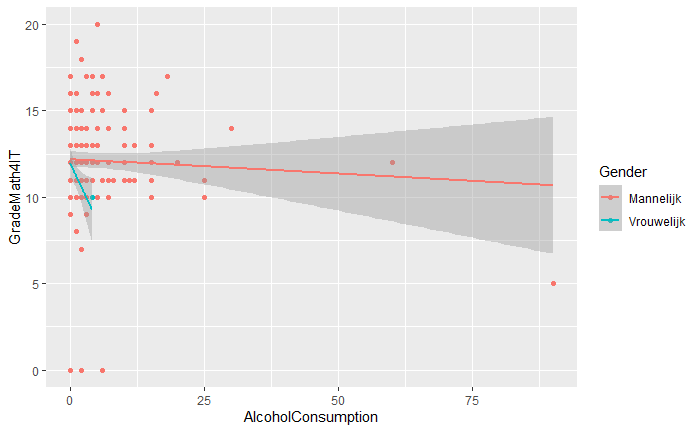
\includegraphics[width=\columnwidth]{AlcMath4IT.png}
    \end{center}
    \caption{Regressie analyse AlcoholConsumption/GradeMath4IT}
    \label{Regressie analyse AlcoholConsumption/GradeMath4IT}
\end{figure}

Ook bij de beschouwing van de correlatie tussen Alcohol Consumption en TestQ1-TestQ15 (Score op de vragen op de wiskundetoets: Niveau 1 – lager onderwijs, Niveau 2 – 1e graad ASO-TSO-BSO en Niveau 3 – 2e graad ASO) werden gelijkaardige resultaten waargenomen.
De correlatiecoëfficiëntwaarde voor mannelijke en vrouwelijke geslachten samen (R) bedraagt -0.054 en de determinatiecoëfficiënt (R$^{2}$) is 0.003. Aangezien de correlatiecoëfficiënt ook tussen -0.3 en 0 ligt en de determinatiecoëfficiënt minder dan 0.1 is, duidt dit op een zeer zwak lineair en dalend verband. Slechts 0,3 procent van de variantie in TestQ1-TestQ15 wordt bepaald door de regressierechte.
Als laatste analyse voor een mogelijke correlatie tussen AlcoholConsumption en GradePOD1 (Welk examencijfer behaalde de student voor Probleemoplossend Denken 1 bij de laatst afgelegde examenkans?) hebben we de volgende resultaten verkregen.
De correlatiecoëfficiëntwaarde voor mannelijke en vrouwelijke geslachten samen (R) bedraagt 0.041 en de determinatiecoëfficiënt (R$^{2}$) is 0.002. Aangezien de correlatiecoëfficiënt tussen -0.3 en 0 ligt en de determinatiecoëfficiënt is minder dan 0.1, duidt dit op een zeer zwak lineair en stijgend verband. Slechts een kleine 0,2 procent van de variantie in GradeMath4IT wordt bepaald door de regressierechte.
Voor mannelijke studenten bedroeg de correlatiecoëfficiëntwaarde (R)  0.032 en de determinatiecoëfficiënt (R$^{2}$) 0.001, duidend op een zeer zwak en stijgend lineair verband. Voor vrouwelijke respondenten bedraagt (R) 0.251 en (R$^{2}$) 0.062 wat duidt op een zeer zwak en stijgend lineair verband.

\begin{figure}[ht]
    \begin{center}
        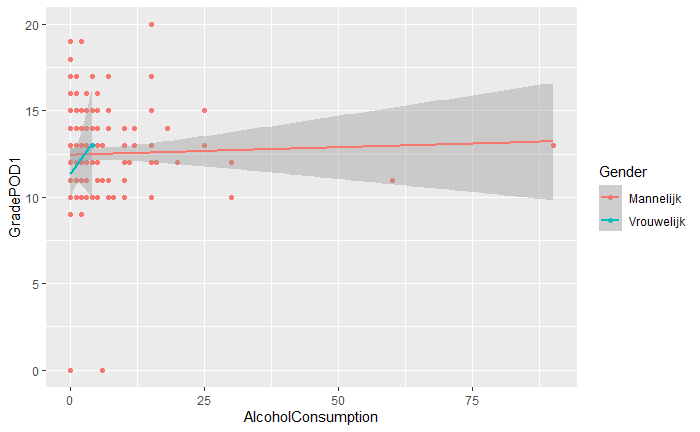
\includegraphics[width=\columnwidth]{AlcPOD.png}
    \end{center}
    \caption{Regressie analyse AlcoholConsumption/GradePOD1}
    \label{Regressie analyse AlcoholConsumption/GradePOD1}
\end{figure}

\subsection{Invloed van sigarettengebruik op wiskundige geletterheid}
Van de deelnemende studenten hebben er 90\% de gegevens meegedeeld van hun resultaten voor Math4IT en het aantal gerookte sigaretten in een week. De meerderheid (162) gaven op niet te roken. De correlatiecoëfficiëntwaarde (R) en de determinatiecoëfficiënt (R$^{2}$) bleken respectievelijk 0.13 en 0.018 te zijn, wat wijst op een zeer zwak verband. De meeste punten liggen op of dicht bij de Y-as waardoor een lineair verband twijfelachtig is. Daarom werd ook een verdeling gemaakt tussen rokers en niet-rokers. Uit de T-test bleek \textit{p} = 0.08622 waardoor de nulhypothese niet verworpen kon worden. De cohens-D waarde bleek \textit{d} = 0.225, wijzend op een kleine effectgrootte en ruim onder de aanbevolen 0.4 van Hattie.


\begin{figure}[ht]
    \begin{center}
        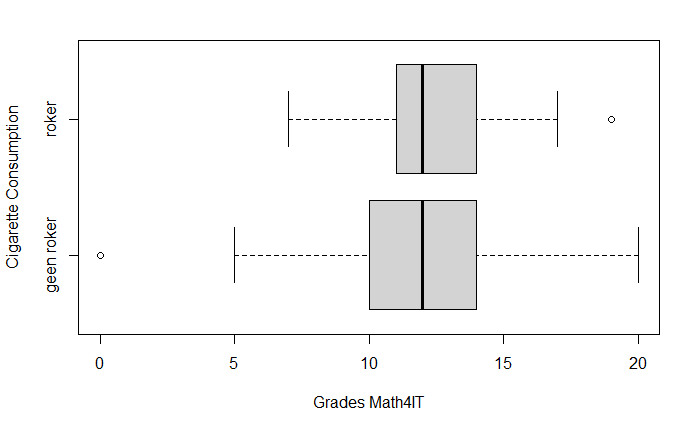
\includegraphics[width=\columnwidth]{CigMath4IT.png}
    \end{center}
    \caption{T-test analyse Cigarette consumption}
    \label{T-test analyse Cigarette consumption}
\end{figure}

De cijfers van probleemoplossend denken 1 en sigarettengebruik werden door 200 studenten opgegeven waarvan 168 niet-rokers zijn. Ook hier kon maar een zeer zwak verband gevonden worden met een R waarde van -0.045 en (R$^{2}$) van 0.002. Een verband dus in negatieve zin. De T-test en cohens-D kwamen respectievelijk uit op 0.098 en \textit{d} = -0.208.
Voor Ongeveer 75\% van alle deelnemers waren zowel de resultaten van de test alsook info over het sigarettenverbuik beschikbaar. 142 keer gaven de studenten op niet te roken. De verdere resultaten liggen in de lijn van de eerder verkregen waardes. R bedroeg -0.110 en (R$^{2}$) 0.012, duidend op een zeer zwak lineair verband. Bij het verschil tussen rokers en niet-rokers kwam de T-test op 0.401 uit, waardoor ook hier geen verband te weerhouden valt. Een waarde van \textit{d} = -0.056 bevestigt dit.



\begin{figure}[ht]
    \begin{center}
        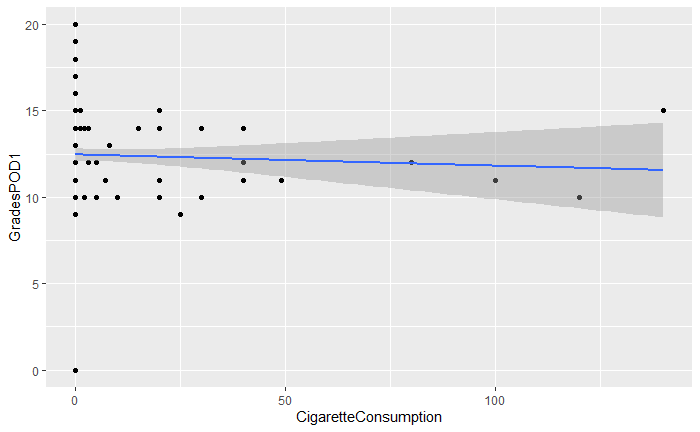
\includegraphics[width=\columnwidth]{CigPOD.png}
    \end{center}
    \caption{Regressie analyse CigaretteConsumption/GradePOD1}
    \label{Regressie analyse CigaretteConsumption/GradePOD1}
\end{figure}

\subsection{Invloed van sporturen op wiskundige geletterheid}
Bij het uitzetten van het aantal sporturen en de resultaten van Math4It stellen we een positieve rechte vast met een hellingsgraad van 0.048. De correlatiecoëfficiëntwaarde (R) en de determinatiecoëfficiënt (R$^{2}$) bleken respectievelijk 0.05 en 0.003 te zijn, wat wijst op zeer zwak verband. Indien we van de 194 ingevulde resultaten een onderscheid maken tussen die van de mannelijke en de vrouwelijke studenten, dan stellen we een positief, zeer zwak verband bij de mannen vast (R = 0.066, (R$^{2}$) = 0.004) en een zeer zwak, negatief verband bij de vrouwelijke deelnemers (R = -0.385, (R$^{2}$) = 0.148). Omdat maar voor 12 studentes gegevens beschikbaar waren, moet dit resultaat met enige nuancering bekeken worden.
Hetzelfde resultaat vinden we terug bij de examenresultaten van POD1. Bij de 183 mannelijke studenten werd een positief, zeer zwak verband gevonden (R = 0.024, (R$^{2}$) = 0.0005), maar bij de 14 vrouwelijke deelnemers een negatief, zeer zwak verband (R = -0.218, (R$^{2}$) = 0.167))
Wanneer we inzoomen op de sporturen en de behaalde resultaten op de test, komen we echter op een omgekeerd resultaat. De 150 mannelijke deelnemers lieten daarbij een negatief, zeer zwak verband optekenen (R = -0.050, (R$^{2}$) = 0.002) terwijl de waarden voor de 13 studentes een positieve, zwakke tendens kende (R = 0.369, (R$^{2}$) = 0.136). Het gaat hier dus om een licht, sterker verband dan bij de vorige resultaten.


\begin{figure}[ht]
    \begin{center}
        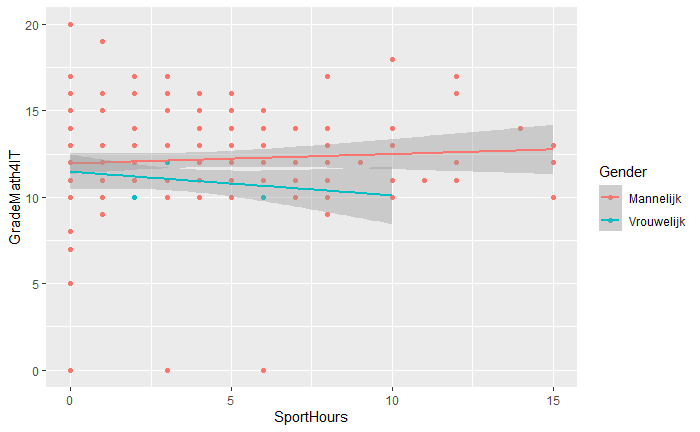
\includegraphics[width=\columnwidth]{SportMath4IT.png}
    \end{center}
    \caption{Regressie analyse SportHours/GradeMath4IT}
    \label{Regressie analyse SportHours/GradeMath4IT}
\end{figure}

\subsection{Invloed van BMI op wiskundige geletterdheid}
We maken bij de analyse gebruik van de body mass index (BMI). Die wordt berekend aan de hand van de volgende formule: \[ BMI = \left(\frac{gewicht}{lengte^2}\right) \] De gerapporteerde resultaten voor Math4It gecombineerd met de BMI-waarden van 190 deelnemers leverde een R waarde van -0.015 op en een determinatiecoëfficiënt van 0.0002. Er is dus sprake van een zeer zwak negatief verband. Een gelijkaardig resultaat merken we op bij het verband met de gerapporteerde eindscores voor het examen van probleem oplossend denken. Daar werd ook een zeer licht negatief verband gevonden met een R waarde van -0.026 en (R$^{2}$) van 0.0007 en dit voor 193 deelnemers. Diezelfde trend stellen we vast bij de cijfers van de test. Een negatieve R waarde van -0.057 en (R$^{2}$) van 0.003 duiden ook hier op een zeer zwak negatief verband.


\begin{figure}[ht]
    \begin{center}
        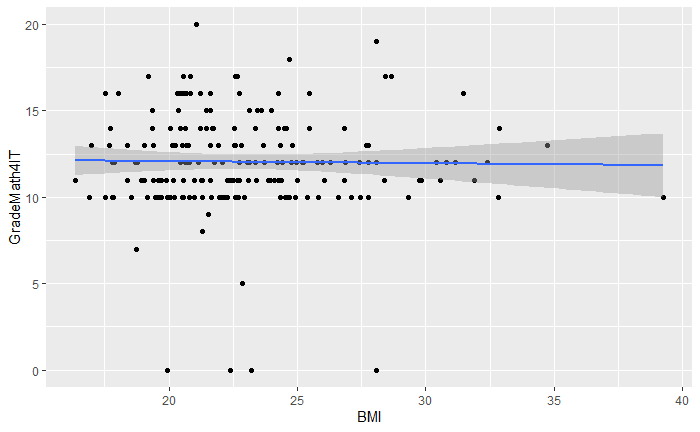
\includegraphics[width=\columnwidth]{BMIMath4IT.png}
    \end{center}
    \caption{Regressie analyse BMI/GradeMath4IT}
    \label{Regressie analyse BMI/GradeMath4IT}
\end{figure}

\section{Conclusie}
Uit de analyse van de invloed van alcoholconsumptie op wiskundige geletterdheid kan opgemaakt worden dat de mate van alcoholconsumptie geen goede voorspeller is voor de resultaten die studenten Toegepaste Informatica behalen op aan wiskunde gerelateerde testen. Dit stemt niet overeen met de bevinding van \textcite{Dielens2013} daar een hogere mate van alcoholgebruik in verband werd gebracht met slechtere examenresultaten.

Vervolgens werd ook geen significant verband gevonden tussen sigarettengebruik en wiskundige geletterdheid. De steekproef was echter niet omvangrijk genoeg om conclusief te zijn (\textit{n} = 33). Daartegenover suggereren \textcite{Kumari2003} dat het roken van sigaretten een positieve impact zou hebben op coginitieve functies die noodzakelijk zijn voor wiskundige taken. Dit werd echter niet bevonden in het huidige onderzoek. Daarnaast werd evidentie gevonden door \textcite{Kalmijn2002} dat roken een negatieve impact zou hebben op het cognitieve vermogen. Opnieuw kan deze studie hiervoor geen evidentie voorleggen.

Voor de invloed van sporturen op wiskundige geletterdheid kon geen verband vastgesteld worden. Dit stemt overeen met de bevinding van \textcite{Dielens2013} en \textcite{Yarkwah2020} daar geen verband werd gevonden tussen fysieke activiteit en wiskundige geletterdheid.

Tot slot bleek uit de analyse geen verband te bestaan tussen BMI en wiskundige geletterdheid. De literatuur suggereert hier echter dat een verhoging in de BMI negatief gecorreleerd zou zijn met de behaalde examenresultaten van studenten \autocite{Dielens2013}. Hier moet echter opgemerkt worden dat niet echter de objectieve meting van de lichaamscompositie een rol speelt, maar ook de zelfperceptie van een individu over zijn gewicht. Een negatieve zelfperceptie zou immers leiden tot lagere scores \autocite{Florin2011}. Dergelijke metingen werden echter niet opgenomen in dit onderzoek.

\subsection{Kritische bedenkingen}
Wiskundige geletterdheid kan moeilijk gedefinieerd worden en wordt immers meebepaald door onderliggende factoren zoals aandachtsvermogen en de efficiëntie en capaciteit van het werkgeheugen. Daarom kan in vraag gesteld worden wat de examentoetsen precies meten die gegeneraliseerd kan worden naar wiskundige geletterdheid. \textcite{Howie2012} stellen eenzelfde probleem vast, daar het geheel aan beschikbare literatuur slechts in geringe mate beschrijft welk abstract concept zij blijken te onderzoeken. Er is in de toekomst nood aan een strakker omlijnd construct. Diezelfde redenering gaat bovendien op voor de BMI, die sterk bekritiseerd is in de literatuur. Mogelijks bestaan er andere constructen die de lichaamscompositie beter omvatten.

Daarnaast was de steekproefpopulatie van vrouwen niet omvangrijk genoeg (\textit{n} = 18) om uitspraken te doen over geslachtsverschillen in de geanalyseerde resultaten. Voor de opleiding Toegepaste Informatica is de proportie aan vrouwelijke studenten enigszins representatief. Het kan interessant zijn om een gelijkaardige studie uit te voeren in een opleiding daar de proportie mannen en vrouwen quasi gelijk zijn.

Tot slot werd opgemerkt dat studenten die niet gestudeerd hebben voor een examen de neiging vertonen om een examen in te dienen zonder invullingen. Dit leidt automatisch tot een nul-score, die de resultaten in de analyse sterk beïnvloedt. In toekomstig onderzoek moet worden opgenomen of de studenten wel degelijk een 0 behaalden of blanco indienden.

%------------------------------------------------------------------------------
% Referentielijst
%------------------------------------------------------------------------------
% TODO: de gerefereerde werken moeten in BibTeX-bestand ``bibliografie.bib''
% voorkomen. Gebruik JabRef om je bibliografie bij te houden en vergeet niet
% om compatibiliteit met Biber/BibLaTeX aan te zetten (File > Switch to
% BibLaTeX mode)

\phantomsection
\printbibliography[heading=bibintoc]

\end{document}

